\documentclass{article}
\usepackage{amsmath}
\usepackage{amsfonts}
\usepackage{lmodern}
\usepackage{mathtools, nccmath}
\usepackage{xparse}
\usepackage{colonequals}

%set mapping
\pagestyle{empty}
\usepackage{tikz}
\usetikzlibrary{calc,trees,positioning,arrows,fit,shapes,calc}

\begin{document}
\title{Word Embedding}
\author{L.J. Brown}
\maketitle

%\newcommand\mat[1]{\mathcal{#1}}
%\newcommand\mat[1]{\boldsymbol{\mathcal{#1}}}
%\newcommand\mat[1]{\boldsymbol{#1}}
\newcommand\mat[3]{\boldsymbol{\mathcal{#1}}_{{#2} \times {#3}}}
\newcommand\mate[1]{\boldsymbol{\mathcal{#1}}}

\newcommand{\N}{\mathbb N}
\newcommand{\Q}{\mathbb Q}

\newcommand*{\logeq}{\ratio\Leftrightarrow}

\DeclarePairedDelimiterX{\set}[1]{\{}{\}}{\setargs{#1}}
\NewDocumentCommand{\setargs}{>{\SplitArgument{1}{;}}m}
{\setargsaux#1}
\NewDocumentCommand{\setargsaux}{mm}
{\IfNoValueTF{#2}{#1} {#1\,\delimsize|\,\mathopen{}#2}}%{#1\:;\:#2}

We outline our first attempt at a method to map all unique words found in a corpus to vectors in a continuous vector space. The hope is that some relationships between words found in the corpus will be preserved through this mapping and will manifest as characteristics of the vector space. The method involves building a co-occurrence matrix from the corpus that represents how frequently word pairs occur together. We then search for word vectors with the soft constraint that given a word vector pair, their inner product will yield a value close to the two values in the co-occurrence matrix associated with those two words. We do this using Stochastic Gradient Descent. The method we outline draws heavily on the implementations by "Word2vec" and "GloVe".

We first map all $n$ unique words found in the corpus, $W = \set {w_1,\ldots ,w_n}$, to integers, $I = \set {1,\,\ldots ,\,n}$, using a function $f$.

%set mapping figure 1
\begin{figure}[h]

	%definitions
	\begin{equation*}
	n \equiv \text{Number of unique words in corpus, } W \equiv \text{Set of unique words in corpus}
	\end{equation*}
	\begin{equation*}
	W = \set {w_1,\ldots ,w_n}
	\end{equation*}
	\begin{equation*}
	I = \set {1,\,\ldots ,\,n}
	\end{equation*}
	
	%mapping equation f : W <-> I
	\begin{equation*}
	f: W \leftrightarrow I
	\end{equation*}
	
 %mapping set figure
 \centering
 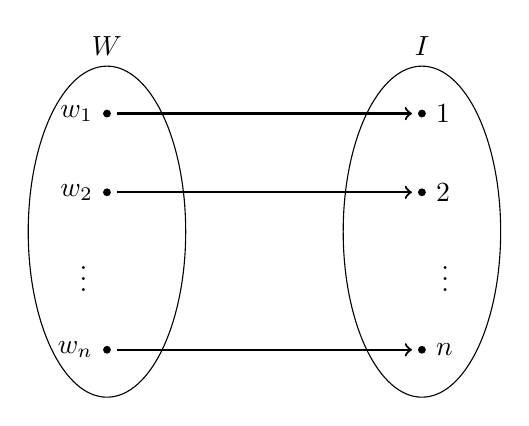
\begin{tikzpicture}[ele/.style={fill=black,circle,minimum width=.8pt,inner sep=1pt},every fit/.style={ellipse,draw,inner sep=-2pt}]
  \node[ele,label=left:$w_1$] (a1) at (0,4) {};    
  \node[ele,label=left:$w_2$] (a2) at (0,3) {};    
  %\node[ele,label=left:$\vdots$] (a3) at (0,2) {};
  \node[label=left:$\vdots$] (a3) at (0,2) {};
  \node[ele,label=left:$w_n$] (a4) at (0,1) {};

  \node[ele,,label=right:$1$] (b1) at (4,4) {};
  \node[ele,,label=right:$2$] (b2) at (4,3) {};
  %\node[ele,,label=right:$\vdots$] (b3) at (4,2) {};
  \node[label=right:$\vdots$] (b3) at (4,2) {};
  \node[ele,,label=right:$n$] (b4) at (4,1) {};

  %\node[draw,fit= (a1) (a2) (a3) (a4),minimum width=2cm] {} ;
  %\node[draw,fit= (b1) (b2) (b3) (b4),minimum width=2cm] {} ; 
  \node[draw,label=above:$W$,fit= (a1) (a2) (a3) (a4),minimum width=2cm] {} ;
  \node[draw,label=above:$I$,fit= (b1) (b2) (b3) (b4),minimum width=2cm] {} ; 
  \draw[->,thick,shorten <=2pt,shorten >=2pt] (a1) -- (b1);
  \draw[->,thick,shorten <=2pt,shorten >=2] (a2) -- (b2);
  %\draw[->,thick,shorten <=2pt,shorten >=2] (a3) -- (b3);
  \draw[->,thick,shorten <=2pt,shorten >=2] (a4) -- (b4);
  
 \end{tikzpicture}
 \caption{Mapping the set of unique words in corpus to a set of integers}
\end{figure}


%Defining Cooccurrence Matrix A
Next we build an $n \times n$ cooccurrence matrix, $\mat{A}{n}{n}$, whose rows and columns correspond to the set of unique words, $W$, and whose elements are the output of a cooccurrence function, $\rho(w_i, w_j)$, which takes words as inputs. For each element, $a_{r_ic_j}$, the words used as inputs for $\rho$ are the words whose integer mappings correspond to the elements row, $r_i$, and column, $c_j$, $\left( f(r_i) = w_i \, \text{and} \, f(c_j) = w_j \right)$.

%Defining Cooccurrence Matrix A
\begin{equation*}
\mat{A}{n}{n}=
\bordermatrix{&c_1&c_2&\ldots &c_n\cr
                r_1&\rho(f(r_1), f(c_1)) &  \rho(f(r_1), f(c_2))  & \ldots & \rho(f(r_1), f(c_n))\cr
                r_2&\rho(f(r_2), f(c_1))  &  \rho(f(r_2), f(c_2)) & \ldots & \rho(f(r_2), f(c_n))\cr
                \vdots& \vdots & \vdots & \ddots & \vdots\cr
                r_4&\rho(f(r_n), f(c_1))  &   \rho(f(r_n), f(c_2))   &\ldots & \rho(f(r_n), f(c_n))}
\end{equation*}

\begin{equation*}
\text{where } a_{ij} = \rho(w_i,w_j)
\end{equation*}

%defining the cooccurrence function, $\rho(w_i, w_j)$
Next we define the cooccurrence function, $\rho(w_i, w_j)$, by first introducing some new variables. For each of the $m$ sentences in the corpus we define $s_i$ as the sequence of words in that sentence. Where $S$ is a sequence containing the $m$ sequences, $s_i, \ldots, s_m$, corresponding to the $m$ sentences of the corpus.

\begin{equation*}
S = \left( s_1, \ldots, s_m \right)
\end{equation*}

For example if the $i^{\text{th}}$ sentence in the corpus is: ``God made mud.'', then the corresponding sequence, $s_i$, in $S$ would be

\begin{equation*}
s_i = \left( \tilde{w_1}, \tilde{w_2}, \tilde{w_3} \right)
\end{equation*}
\begin{equation*}
\text{where } \tilde{w_1}, \tilde{w_2}, \tilde{w_3} \, \epsilon \, W
\end{equation*}

Then we define a distance function, $d(s_i, \set{\tilde{w_j}, \tilde{w_k}})$, whose parameters are a sequence of words, $s_i$, in $S$ (corresponding to a sentence of the corpus) and a set or an unordered pair of words that are members of the sequence $s_i$. The distance function, $d(s_i, \set{\tilde{w_j}, \tilde{w_k}})$, returns a value one more than the number of words between the word pair, $\set{\tilde{w_j}, \tilde{w_k}}$, in sentence corresponding to the sequence, $s_i$.

\begin{equation*}
d(s_i, \set{\tilde{w_j}, \tilde{w_k}}) = \mid j - k \mid
\end{equation*}

Finally we define the cooccurrence function, $\rho(\tilde{w_i}, \tilde{w_j})$, as

\begin{equation*}
\rho(w_i,w_j) = 
\begin{cases}
0, \, \text{if} \, w_i = w_j
\\
\sum_{s \epsilon S} { \sum_{p \epsilon \set{[s]^2} } {
\begin{cases}
\log \left(\frac{1}{d(s,p)} \right), \, \text{if} \, w_i, w_j \, \epsilon \, p
\\
0, \, \text{otherwise}
\end{cases}
} }, \, otherwise
\end{cases}
\end{equation*}
\begin{equation*}
\text{Where } \set{[s_i]^2} \text{is the set of all unordered pairs of words in the sequence } s_i . 
\end{equation*}
Stated simply, $\rho(w_i, w_j)$ finds all times that the words $w_i$ and $w_j$ appear together in sentences of the corpus, and sums the $\log \left( \frac{1}{\text{their distance apart}} \right)$. Note that the value of the cooccurrence function, $\rho(w_i, w_j)$, when the two inputs are the same word is zero. This corresponds to the diagonal entries of the cooccurrence matrix $\mate{A}$. The matrix $\mate{A}$ will also be symmetric about its diagonal due to the property of $\rho(w_i, w_j)$ that,

\begin{equation*}
\rho(w_i,w_j) = \rho(w_j,w_i)
\end{equation*}
therefore,
\begin{equation*}
a_{ij} = a_{ji}, \, \text{in the matrix } \, \mate{A}.
\end{equation*}


%defining n word vectors of dimensionality d
%Defining soft constraint of equality
Next we search for a set of $n$ word vectors, $\vec{w}_{i},\ldots ,\vec{w}_{n}$ , of dimensionality $v$ that best satisfy the condition that the inner product between any two word vectors is a value close to the two elements in matrix $\mate{A}$ corresponding to the two words intersection. We exclude the diagonal elements from meeting this condition which correspond to the intersection of one word with itself. We will represent the desired $n$ word vectors as the column vectors of a matrix $\mat{W}{v}{n}$.

  \begin{align*}
    \mat{W}{v}{n} &= \begin{pmatrix}
    	\begin{bmatrix} \vec{w}_{1} \end{bmatrix} , \ldots , \begin{bmatrix} \vec{w}_{n}\end{bmatrix}
	 \end{pmatrix}
  \end{align*}

%margin note
\marginpar{The objective function, $J$, iterates over just the upper triangular section of the matrix $\mate{A}$ instead of both the lower and upper triangular sections due to its symmetric properties. We choose to iterate with the column values, $c$, changing the fasted due to the way most operating systems load memory into ram.}

In order to formally define the properties of the word vectors we wish to find, we write a set of $\frac{n^2 - n}{2}$ soft constraints, $C = \set{c_{12},c_{13},\cdots ,c_{n \choose 2}}$, as
\begin{equation*}
c_{ij} \equiv \vec{w}_{i}^T \cdot \vec{w}_{j} \logeq a_{ij} \text{, where $i \neq j$.}
\end{equation*}

\begin{equation*}
\text{where } \frac{n^2 - n}{2} \text{ is the number of non-diagonal elements in the matrix } \mate{A}.
\end{equation*}
Or more intuitively $\frac{n^2 - n}{2} = \frac{2(n!)}{2!(n-2)!} = 2 {n \choose 2 }$ is two times the number of ways you can combine the $n$ word vectors in pairs of $2$ with no repetition. However, order does not matter for the constraints when taking the inner product of two word vectors as $\mate{A}$ is symmetric about its diagonal and 

\begin{equation*}
\vec{w}_{i}^T \cdot \vec{w}_{j} = \vec{w}_{j}^T \cdot \vec{w}_{i}
\end{equation*}

\begin{equation*}
a_{ij} = a_{ji}
\end{equation*}


%Error function between two word vectors
\text{We define an error function, $\varepsilon$, between two word vectors, $\vec{w}_{i}$ and $\vec{w}_{j}$, as}
\begin{equation*}
\varepsilon(i,j) = \vec{w}_{i}^T \cdot \vec{w}_{j} - a_{ij}
\end{equation*}
\begin{equation*}
\text{where $a_{ij}$ is an element in the Matrix $\mate{A}$}
\end{equation*}

%Objective function J for entire dataset
The method we choose to find the values of the matrix $\mate{W}$ is \textbf{Stochastic Gradient Descent}. We define an objective function, $J$, to minimize as
\begin{equation*}
J = \frac{1}{2 {n \choose 2} } \sum_{r=1}^{n}{\sum_{c=r+1}^{n}{
\begin{cases}
\varepsilon(r,c)^2, \, if \, r \neq c
\\
0, \, otherwise
\end{cases}
}}
\end{equation*}

When $J$ is at a minimum then the column vectors of $\mate{W}$ will best meet our set of soft constraints, $C$.

%Defining an objective function for a specific word vector
We next define an individual objective function for each word vector, $J_{\vec{w}_{i}}$. During the optimization process, and during each iteration, we randomly select a column vector of $\mate{W}$, $\vec{w_i}$, to update by computing the gradient of the chosen individual word vector, $\frac{\partial J_{\vec{w}_{i}}}{\partial \vec{w}_{i}}$. We define the objective function for an individual word vector, $\vec{w}_{i}$,  as
\begin{equation*}
J_{\vec{w}_{i}} = \frac{1}{2} \sum_{j=1}^{n} {\begin{cases}
\varepsilon(i,j)^2, \, if \, i \neq j
\\
0, \, otherwise
\end{cases}}
\end{equation*}

And compute the gradient of that specific objective function, $\frac{\partial J_{\vec{w}_{i}}}{\partial \vec{w}_{i}}$, as
%Defining the gradient for an individual word vectors objective function
\begin{equation*}
\frac{\partial J_{\vec{w}_{i}}}{\partial \vec{w}_{i}} = \sum_{j=1}^{n}{\begin{cases}
\vec{w}_{i} \, \odot \, \left( \vec{w}_{i}^T \cdot \vec{w}_{j} - y_{ij} \right), \, if \, i \neq j
\\
0, \, otherwise
\end{cases}}
\end{equation*}

%iteration updation for random word vector
The optimization process in pseudo code is outlined bellow:
$\\\\ n \equiv \text{Number of unique words in corpus}$
$\\ m \equiv \text{Number of training iterations}$
$\\ \eta \equiv \text{Learning rate}$

\begin{equation*}
\text{For $i = 1,2, \ldots , m$, do:}
\end{equation*}
\begin{equation*}
x := \text{random number range} [1,n]
\end{equation*}
\begin{equation*}
\vec{w}_{x} := \vec{w}_{x} - \eta \frac{\partial J_{\vec{w}_{x}}}{\partial \vec{w}_{x}}
\end{equation*}

\end{document}